\documentclass{article}

%? Pakete für Sprache und Layout
\usepackage[ngerman]{babel}
\usepackage[a4paper, left=3cm, right=3cm, top=2.5cm, headheight=110pt]{geometry}

%? Pakete für Aufgaben
\usepackage{colortbl}
\usepackage{graphicx}
\usepackage{subcaption}


%? Pakete für Optik
\usepackage{cmbright}
\usepackage[OT1]{fontenc}
\usepackage{enumitem}
\usepackage{fancyhdr}
\usepackage{csquotes}


% Kopfzeile
\pagestyle{fancy}
\fancyhead[L]{Einführung in \LaTeX \\ Übung 5}
\fancyhead[C]{{Gleitumgebung}\\}
\fancyhead[R]{Adrian Riedel \\ 9. März 2022}


\begin{document}
\section*{Übung 5.1: Bunte Tabelle}
\begin{enumerate}[label=\alph*)]
    \item Eine Tabelle mit farbigen Zellen aus dem Package \emph{colortbl}
          \begin{table}[h]
              \caption{Hier kommt die vielsagende Beschriftung und die sagt: \\ \enquote{Das ist eine Tabelle, die wo eine blaue linke Spalte haben tut und die erste Reihe grau sein tut.}}
              \begin{tabular}{>{\columncolor{blue} \color{white}}l|l}
                  \rowcolor[gray]{.5} \color{black} Wochentag & Buchstaben \\
                  Montag                                      & 6          \\
                  Dienstag                                    & 8          \\
                  Mittwoch                                    & 8          \\
                  Donnerstag                                  & 10         \\
                  Freitag                                     & 7          \\
                  Samstag                                     & 7          \\
                  Sonntag                                     & 7
              \end{tabular}
          \end{table}
\end{enumerate}

\section*{Übung 5.2: Abbildungen}
\begin{enumerate}[label=\alph*)]
    \item Ein Bild
          \begin{figure}[h]
              \includegraphics[width=3cm, angle=69]{vi-icon2.png}
              \caption{Icon der VInf Stundenplan App (gedreht)}
          \end{figure}
    \item Zwei Bilder
          \begin{figure}[h]
              \begin{subfigure}{.5\textwidth}
                  \includegraphics[height=3cm]{bob.png}
                  \caption{Bob kann das schaffen}
              \end{subfigure}
              \begin{subfigure}{.5\textwidth}
                  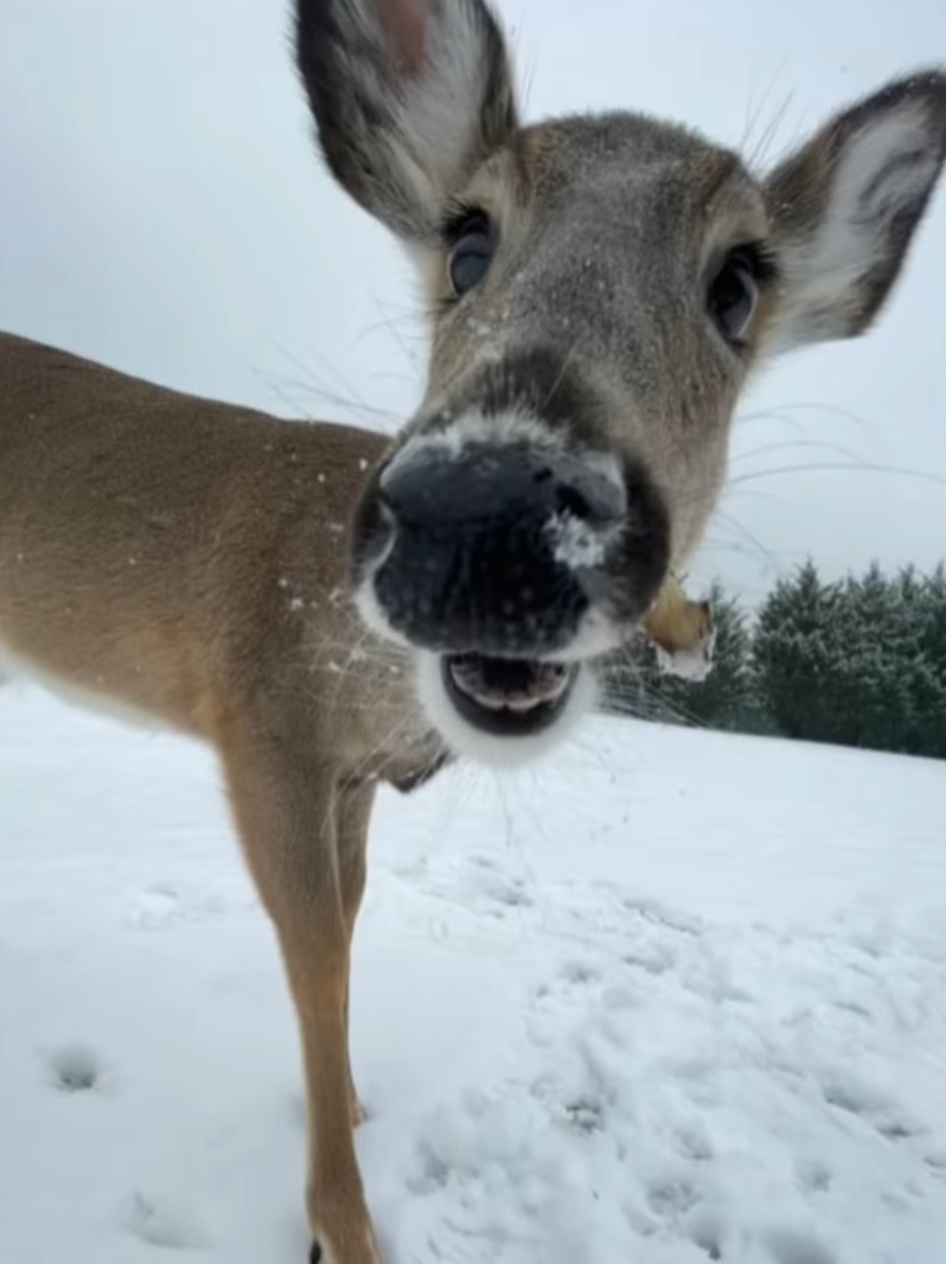
\includegraphics[height=3cm, width=7cm, keepaspectratio=false]{andrehas.jpg}
                  \caption{wide Andrehas}
              \end{subfigure}
              \caption{Bob mag Rehe}
          \end{figure}
\end{enumerate}


\end{document}